\documentclass[12pt,a4paper]{exam}

\usepackage[utf8]{inputenc}
\usepackage[T1]{fontenc}
\usepackage{amsmath}
\usepackage{amsfonts}
%\usepackage{amssymb}
\usepackage{graphicx}
\usepackage{geometry}
\usepackage{cancel}
\usepackage{enumitem}

\geometry{a4paper, margin=2cm}

\newcommand{\ito}{It$\hat{o}$}
\newcommand{\expect}[1]{\mathbb{E}^\mathbb{#1}}
\newcommand{\expectt}[2]{\mathbb{E}_{#2}^\mathbb{#1}}

\usepackage{cprotect}

\usepackage{xcolor}
\definecolor{maroon}{cmyk}{0, 0.87, 0.68, 0.32}
\definecolor{halfgray}{gray}{0.55}
\definecolor{ipython-frame}{RGB}{207, 207, 207}
\definecolor{ipython-bg}{RGB}{247, 247, 247}
\definecolor{ipython-red}{RGB}{186, 33, 33}
\definecolor{ipython-green}{RGB}{0, 128, 0}
\definecolor{ipython-cyan}{RGB}{64, 128, 128}
\definecolor{ipython-purple}{RGB}{170, 34, 255}
\usepackage{listings}
\lstdefinelanguage{iPython}{
	morekeywords={access,and,del,except,exec,in,is,lambda,not,or,raise},
	morekeywords=[2]{for,print,abs,all,any,basestring,bin,bool,bytearray,callable,chr,classmethod,cmp,compile,complex,delattr,dict,dir,divmod,enumerate,eval,execfile,file,filter,float,format,frozenset,getattr,globals,hasattr,hash,help,hex,id,input,int,isinstance,issubclass,iter,len,list,locals,long,map,max,memoryview,min,next,object,oct,open,ord,pow,property,range,reduce,reload,repr,reversed,round,set,setattr,slice,sorted,staticmethod,str,sum,super,tuple,type,unichr,unicode,vars,xrange,zip,apply,buffer,coerce,intern,elif,else,if,continue,break,while,class,def,return,try,except,import,finally,try,except,from,global,pass, True, False},
	sensitive=true,
	morecomment=[l]\#,%
	morestring=[b]',%
	morestring=[b]",%
	moredelim=**[is][\color{black}]{@@}{@@},
	%%
	%morestring=[s]{'''}{'''},% used for documentation text (mulitiline strings)
	%morestring=[s]{"""}{"""},% added by Philipp Matthias Hahn
	%%
	%morestring=[s]{r'}{'},% `raw' strings
	%morestring=[s]{r"}{"},%
	%morestring=[s]{r'''}{'''},%
	%morestring=[s]{r"""}{"""},%
	%morestring=[s]{u'}{'},% unicode strings
	%morestring=[s]{u"}{"},%
	%morestring=[s]{u'''}{'''},%
	%morestring=[s]{u"""}{"""}%
	%
	% {replace}{replacement}{lenght of replace}
	% *{-}{-}{1} will not replace in comments and so on
	%literate=
	%{\%}{{{\color{ipython-purple}+}}}1,
	%{�}{{\'a}}1 {�}{{\'e}}1 {�}{{\'i}}1 {�}{{\'o}}1 {�}{{\'u}}1,
	%{�}{{\'A}}1 {�}{{\'E}}1 {�}{{\'I}}1 {�}{{\'O}}1 {�}{{\'U}}1
	%{�}{{\`a}}1 {�}{{\`e}}1 {�}{{\`i}}1 {�}{{\`o}}1 {�}{{\`u}}1
	%{�}{{\`A}}1 {�}{{\'E}}1 {�}{{\`I}}1 {�}{{\`O}}1 {�}{{\`U}}1
	%{�}{{\"a}}1 {�}{{\"e}}1 {�}{{\"i}}1 {�}{{\"o}}1 {�}{{\"u}}1
	%{�}{{\"A}}1 {�}{{\"E}}1 {�}{{\"I}}1 {�}{{\"O}}1 {�}{{\"U}}1
	%{�}{{\^a}}1 {�}{{\^e}}1 {�}{{\^i}}1 {�}{{\^o}}1 {�}{{\^u}}1
	%{�}{{\^A}}1 {�}{{\^E}}1 {�}{{\^I}}1 {�}{{\^O}}1 {�}{{\^U}}1
	%{�}{{\oe}}1 {�}{{\OE}}1 {�}{{\ae}}1 {�}{{\AE}}1 {�}{{\ss}}1
	%{�}{{\c c}}1 {�}{{\c C}}1 {�}{{\o}}1 {�}{{\r a}}1 {�}{{\r A}}1
	%{�}{{\EUR}}1 {�}{{\pounds}}1
	%
	%{^}{{{\color{ipython_purple}\^{}}}}1
	%{=}{{{\color{ipython_purple}=}}}1
	%%
	%*{-}{{{\color{ipython_purple}-}}}1
	%{*}{{{\color{ipython_purple}$^\ast$}}}1
	%{/}{{{\color{ipython_purple}/}}}1%%
	%{+=}{{{+=}}}1
	%{-=}{{{-=}}}1
	%{*=}{{{$^\ast$=}}}1
	%{/=}{{{/=}}}1,
	%
	identifierstyle=\color{black}\footnotesize\ttfamily,
	commentstyle=\color{ipython-cyan}\footnotesize\itshape\ttfamily,
	stringstyle=\color{ipython-red}\footnotesize\ttfamily,
	keepspaces=true,
	showspaces=false,
	showstringspaces=false,
	rulecolor=\color{ipython-frame},
	frame=single,
	frameround={t}{t}{t}{t},
	%framexleftmargin=6mm,
	%numbers=left,
	%numberstyle=\color{ipython-cyan},
	backgroundcolor=\color{ipython-bg},
	%   extendedchars=true,
	basicstyle=\footnotesize\ttfamily,
	keywordstyle=[2]\color{ipython-green}\bfseries\footnotesize\ttfamily, 
	keywordstyle=\color{ipython-purple}\bfseries\footnotesize\ttfamily
}

\lstdefinelanguage{iOutput} {
	sensitive=true,
	identifierstyle=\color{black}\small\ttfamily,
	stringstyle=\color{ipython-red}\small\ttfamily,
	keepspaces=true,
	showspaces=false,
	showstringspaces=false,
	rulecolor=\color{ipython-frame},
	%frame=single,
	%frameround={t}{t}{t}{t},
	%backgroundcolor=\color{ipython-bg},
	basicstyle=\small\ttfamily,
}

\lstnewenvironment{ipython}[1][]{\lstset{language=iPython,mathescape=true,escapeinside={*@}{@*}}%
}{%
}

\lstnewenvironment{ioutput}[1][]{\lstset{language=iOutput,mathescape=true,escapeinside={*@}{@*}}%
}{%
}


\title{Advanced Financial Modeling Course 23/24\\ Exam}
\author{Prof. Andrea Carapelli, Prof. Matteo Sani}
\date{$16^{\mathrm{th}}$ February 2024}

\printanswers
%\noprintanswers
\begin{document}
\maketitle
\addpoints{exam}
\begin{center}
\fbox{\fbox{\parbox{5.5in}{\centering
Answer the questions in the spaces provided. If you run out of room for an answer, continue on the page back.}}}
\end{center}

\begin{center}
\vspace{5mm}
\makebox[0.75\textwidth]{Student's name:\enspace\hrulefill}
\end{center}

\section*{Questions}
\vspace{.5cm}
\begin{questions}

%%%%%%%%%%%%%%%%%%%%%%%%%%%%%%%%%%%%%%%%%%%%%%%%%%%%
\question The 1-year spot rate on US treasury bonds is 9\%, the 2-year spot rate is 9.5\% and the 3-year spot rate is 10\%. 
\begin{itemize}
\item Calculate the implied 1-year ahead, 1-year forward rate, $F(0;1,2)$. Explain why a 1-year forward rate of 9.6\% could not be explained by the market;
\item calculate the forward rates  $F(0; 2, 3$ and $F(0; 1,3)$. Is there a link between $F(0;1,2),F(0;2,3)$ and $F(0;1,3)$ ?
\end{itemize}
\begin{solution}
\begin{itemize}
\item The forward rates are as follows:
\begin{equation}
F(0;1,2)= \cfrac{0.095*2 - 0.09*1}{2-1} = 0.1, \quad F(0;2,3)= \cfrac{0.1*3 - 0.095*2}{3-2} = 0.11, \quad F(0;1,3)= \cfrac{0.1*3 - 0.09*1}{3-1} = 0.105
\end{equation}
If you lend €100 at $t=1$ at 9.6\%, your cash flow is -€100 at $t=1$ and €109.6 at $t=2$. You can do better by borrowing now for 1 year $€100/1.09=€91.74$ and lending the same amount for 2 years. Your net cash flow is then €0 at $t=0$, -€100 at $t=1$ (that is $€91.74\cdot 1.09$), and €110 at $t=2$ (that is $€91.74\cdot 1.095^2$). Compared to the first option, you have thus a certain higher cash flow at $t=2$: €110 vs. €109.6.  There is then no reason to accept the 9.6\% rate contract. 
\item The link between the forward rate is as follows:
\begin{equation}
\cfrac{(1+F(0;1,3)^2}{1+F(0;1,2)} = \cfrac{(1+r_3)^3}{(1+r^2)} \Rightarrow (1+F(0;1,3)^2 = (1+F(0;1,2))(1+F(0;2,3))
\end{equation}
Hence, with any two of three forward rates, you can deduct the third one.
\end{itemize}
\end{solution}

%%%%%%%%%%%%%%%%%%%%%%%%%%%%%%%%%%%%%%%%%%%%%%%%%%%%%
\question If the pure expectations hypothesis holds, why might the yield curve be flat, upward sloping, or downward sloping? The government implements a credible “tight” monetary policy by raising short-term (e.g. 3-month) interest rates. How could this affect the yield curve?
\begin{solution}
A flat yield curve means that the market expects the rates to be constant.
The interpretation of a monotonically upward sloping yield curve depends on the slope. For instance, consider that the 1-year, 2-year and 3-year YTM are respectively 4\%, 5\% and 6\%. Then the forwards are $F(0;1,2)=6\%$, $F(0;2,3)=8\%$ meaning that the rates are expected to grow monotonically. If instead, the 1-year, 2-year and 3-year YTM are for instance  4\%, 5\% and 5.1\%. Then the forward are $F(0;1,2)=6\%'$, $F(0;2,3)=5.3\%$ meaning that the rates are \textbf{not} expected to grow monotonically. 
The same reasoning holds for a downward sloping yield curve.
\end{solution}
%%%%%%%%%%%%%%%%%%%%%%%%%%%%%%%%%%%%%%%%%%%%%%%%%%%%%
\question A bank offers to borrow €100 from you at an interest rate applicable between the end of year 1 and the end of year 2 at a rate of 13\% (i.e. the forward rate). The spot rates for 1-year and 2-year are currently 10\% and 12\% respectively. Explain whether you would take the bank’s offer. 
\begin{solution}
The forward rate between year 1 and year 2 is $F(0;1,2)=14\%$. It is then easy to show that it is irrational to accept lending at 13\% at year 1. Indeed, if you lend €100 at $t=1$ at 13\%, your cash flow is -€100 at $t=1$ and €113 at $t=2$. 
You can do better by borrowing now for 1 year $€100/1.10=€90.91$ and lend the same amount for 2 years. Your net cash flow is then €0 at $t=0$, -€100 at $t=1$ ($€90.91\cdot 1.10$), and €114.04 at $t=2$ (that is $90.91\cdot 1.12^2$). 
Compared to the first option, you have thus a certain higher cash flow at $t=2$: 114 vs. 113.  There is then no reason for the lender to accept the 13\% rate contract. 
\end{solution}
%%%%%%%%%%%%%%%%%%%%%%%%%%%%%%%%%%%%%%%%%%%%%%%%%%%%%

\question Companies A and B have been offered the following rates per annum on a 20 million 5-year loan:
\begin{center}
\begin{tabular}{|c|c|c|}
\hline
& Fixed rate & Floating rate \\ \hline
Company A &  5.0\% & LIBOR+0.1\% \\ \hline
Company B & 6.4\% & LIBOR+0.6\%  \\ \hline
\end{tabular}
\end{center}

Company A requires a floating-rate loan; company B requires a fixed-rate loan. Design a swap that will net a bank, acting as intermediary, 0.1\% per annum and that will appear equally attractive to both companies.
\begin{solution}
A has an apparent comparative advantage in fixed-rate markets but wants to borrow floating. B has an apparent comparative advantage in floating-rate markets but wants to borrow fixed. This provides the basis for the swap. There is a 1.4\% per annum differential between the fixed rates offered to the two companies and a 0.5\% per annum
differential between the floating rates offered to the two companies. The total gain to all parties from the swap is therefore 1.4-0.5 = 0.9\% per annum. Because the bank gets 0.1\% per annum of this gain, the swap should make each of A and B 0.4\% per
annum better off. This means that it should lead to A borrowing at LIBOR -0.3\% and to B borrowing at 6\%. 
\end{solution}

\question A 100 million interest rate swap has a remaining life of 10 months. Under the terms of the swap; 6-month LIBOR is exchanged for 7\% per annum (compounded semiannually). The average of the bid-offer rate being exchanged for 6-month LIBOR in swaps of all maturities is currently 5\% per annum with continuous compounding. The 6-month LIBOR rate was 4.6\% per annum 2 months ago. What is the current value of the swap to the party paying floating ? What is its value to the party paying fixed ?

\begin{solution}
In four months 6 million ($0.5\times 0.12\times 100$~million) will be received and 4.8 million ($0.5\times 0.096\times 100$~million) will be paid. (We ignore day count issues.) In 10 months 6 million will be received, and the LIBOR rate prevailing in four months-time will be paid. The value of the fixed-rate bond underlying the swap is
\begin{equation*}
6 \exp(-0.1 \times 4/12) + 6 \exp(0.1\times  10/12) = 103.328 \text{million}
\end{equation*}
The value of the floating-rate bond underlying the swap is 
\begin{equation*}
(100 + 4:8) \exp(0.1\times  4/12) = 101364 \text{million}
\end{equation*}
The value of the swap to the party paying floating is $103328-  101364 = 1964$~million. 
The value of the swap to the party paying fixed is the opposite. 

These results can also be derived by decomposing the swap into forward contracts. Consider the party paying floating. The first forward contract involves paying 4.8~million and receiving 6~million in four months. It has a value of $1.2e^{-0.1\cdot 4/12} = 1.161$~million.
To value the second forward contract, we note that the forward interest rate is 10\% per annum with continuous compounding, or 10.254\% per annum with semiannual compounding. The value of the forward contract is
\begin{equation*}
100\times  (0.12\times 0.5-0.10254\times 0.5)e^{-0.1\cdot 10/12} = 0.803 \text{million}
\end{equation*}

The total value of the forward contract is therefore $1.161 + 0.803 = 1.964$~million.
\end{solution}

\question  A financial institution has entered into an interest rate swap with company A. Under the terms of the swap, it receives 10\% per annum and pays 6-month LIBOR on a principal of 10 million for 5 years. Payments are made every 6 months. 
Suppose that company A defaults on the sixth payment date (at the end of year 3) when the interest rate (with semiannual compounding) is 8\% per annum for all maturities. 
What is the loss to the financial institution ? Assume that 6-month LIBOR was 9\% per annum halfway through year 3. 
Use LIBOR discounting.

\begin{solution}
At the end of year 3 the financial institution was due to receive 500000 and pay 450000. The immediate loss is therefore 50000.

To value the remaining swap we assume that forward rates 
rates are 8\% per annum. The remaining cash flows are therefore valued on the assumption that the floating payment is and the net payment that would be received is . The
total cost of default is therefore the cost of foregoing the following cash flows:
\begin{center}
	\begin{tabular}{|l|l|}
	\hline
	3 year & 50000 \\ \hline
	3.5 year & 100000 \\ \hline
	4 year &  100000 \\ \hline
	4.5 year & 100000 \\ \hline
	5 year & 100000 \\ \hline
	\end{tabular}
\end{center}
Discounting these cash flows to year 3 at 4\% per six months, we obtain the cost of the default as 413000.
\end{solution}

\question A currency swap has a remaining life of 15 months. It involves exchanging interest at 10\% on 20 million for interest at 6\% on 30 million once a year. The term structure of interest rates in both the United Kingdom and the United States is currently flat,
and if the swap were negotiated today the interest rates exchanged would be 4\% in dollars and 7\% in sterlings. All interest rates are quoted with annual compounding. The current exchange rate (dollars per pound sterling) is 1.8500. What is the value of the swap to the party paying sterling ? What is the value of the swap to the party paying dollars ?

\begin{solution}
The swap involves exchanging the sterling interest of $20\cdot 0.14 = 2.8$~million for the dollar interest of $30\cdot 0.1 = 3$~million. 
The principal amounts are also exchanged at the end of the life of the swap. The value of the sterling bond underlying the swap is
$2.8(1.11)^{-0.25} + 22.8(1.11)^{-5/4} = 22.739$~million pounds.

The value of the dollar bond underlying the swap is $3(1.08)^{-0.25} + 33(1.08)^{-5/4} = 32.916$~million.

The value of the swap to the party paying sterling is therefore
-4.604 million.

The results can also be obtained by viewing the swap as a portfolio of forward contracts. The continuously compounded interest rates in sterling and dollars are 10.436\% per annum and 7.696\% per annum. The 3-month and 15-month forward exchange rates are
$1:65e^{-(0.10436-0.07696)0.25}= 1.6387$ and $1.65e^{-(0:10436-0.07696)1.25} = 1.5944$.
The values of the two forward contracts corresponding to the exchange of interest for the party paying sterling are therefore
$(3-2.8\times  1.6387) e^{-0.07696*0.25} = -2.558$~ million
and $(3- 2.8\times  1.5944) e^{-0.07696*1:25} = 1.330$~million.
The value of the forward contract corresponding to the exchange of principals is $(30-20\times 1.5944) e^{-0.07696*1:25} = -1.716$~million.
The total value of the swap is $1.558-1.330-1.716 = 4.604$~million.
\end{solution}

\question A financial institution has entered into a 10-year currency swap with company A.
Under the terms of the swap, the financial institution receives interest at 3\% per annum in Swiss francs and pays interest at 8\% per annum in US dollars. Interest payments are exchanged once a year. The principal amounts are 7 million dollars and 10 million
francs. Suppose that company A declares bankruptcy at the end of year 6, when the exchange rate is 0.80 dollars per franc. What is the cost to the financial institution ? Assume that, at the end of year 6, the interest rate is 3\% per annum in Swiss francs and 8\%
per annum in US dollars for all maturities. All interest rates are quoted with annual compounding.

\begin{solution}
When interest rates are compounded annually
\begin{equation*}
	F_0 = S_0\left(\cfrac{1+r}{1+r_f}\right)^T
\end{equation*}
where $F_0$ is the T-year forward rate, $S_0$ is the spot rate, $r$ is the domestic risk-free rate, and $r_f$ is the foreign risk-free rate. As $r = 0.08$ and $r_f = 0.03$, the spot and forward
exchange rates at the end of year 6 are

\begin{center}
	\begin{tabular}{|l|l|}
\hline
Spot & 0.8000 \\ \hline
1 year forward & 0:8388 \\ \hline
2 year forward & 0:8796 \\ \hline
3 year forward & 0:9223 \\ \hline
4 year forward & 0:9670 \\ \hline
	\end{tabular}
\end{center}

The value of the swap at the time of the default can be calculated on the assumption that forward rates are realized. The cash flows lost as a result of the default are therefore as follows:

\begin{center}
	\begin{tabular}{|c|c|c|c|c|c|}
\hline
Year & Dollar& Sw Fr & Forward &Dollar Equivalent. & Loss \\ \hline
6 &560000& 300000& 0.8000& 240000 & (320000) \\ \hline
7 &560000& 300000& 0.8388& 251000 & (308400) \\ \hline
8 &560000& 300000& 0.8796& 263900 & (296100) \\ \hline
9 &560000& 300000& 0.9223& 276700 & (283300) \\ \hline
10& 7560000& 10300000& 0.9670& 9960100 & 2400100 \\ \hline
	\end{tabular}
\end{center}

Discounting the numbers in the final column to the end of year 6 at 8\% per annum, the cost of the default is 679800. Note that, if this were the only contract entered into by company B, it would make no sense for the company to default at the end of year six as the exchange of payments. At that time has a positive value to company B.
In practice company B is likely to be defaulting and declaring bankruptcy for reasons unrelated to this particular contract and payments on the contract are likely to stop when bankruptcy is declared.
\end{solution}

\question Assume that company A has agreed to pay a 6-month Libor and receive a fixed interest rate of 8\% per annum (with interest payable every six months) from the face value of 100 million. Swap is 1.25 years to expire. The interest rates for 3, 9 and 15 months are: 10\%, 10.5\% and 11\% respectively. Assume that interest rates are continously compounded. The 6-month Libor is currently 10.2\%. Calculate the value of this swap for company A.

\begin{solution}
In our case: $Q= 100$~mln - the principal of the swap (in bond notation it is face value FV), LIBOR=0.102 - 6 months LIBOR, T=1.25 - the maturity of the bond as a fraction of the year (15 months is 1.25 of year), r3m=0.10 - 3 months interest rate, r9m=0.105 - 9 months interest rate, r15m=0.11 - 15 months interest rate, rfix=0.08 - fixed interest rate, 2 - number of payments in a year

Since the company A pays floating interest and receives fixed one
\begin{equation*}
V=V_{fix}-V_{fl} = \sum_{i=1}^n \cfrac{k}{e^{r_i t_i}} + \cfrac{Q}{e^{r_n t_n}} - \cfrac{k^*}{e^{r_1 t_1}}+\cfrac{Q}{e^{r_1 t_1}}
\end{equation*}

The fixed leg value is
\begin{equation*}
V_{fix} = 4e^{-0.25\cdot 0.1} +  4e^{-0.75\cdot 0.105} +  104e^{-1.25\cdot 0.11} = 98.25\text{mln}
\end{equation*}

The floating payment is based on LIBOR and the nearest (first) payment is 
\begin{equation*}
k^*=0.102\cdot0.5\cdot 100 = 5.1\text{mln}
\end{equation*}
Hence:
\begin{equation*}
V_{fl}=5.1e^{-0.25\cdot 0.1}+100\cdot e^{-0.25\cdot 0.1} = 102.51
\end{equation*}

And the final calcualtion
\begin{equation*}
V = 98.24-102.51=-4.27\text{mln}
\end{equation*}
which is the swap value for company A.
\end{solution}

\question Determine the value of the swap from previous exercise in the way as described in the Relationship between interest rate swap and FRA part.
\begin{solution}
The cash flows that will be exchanged after three months can be calculated at the beginning. The interest rate of 8\% will be exchanged for a rate of 10.2\%. Let us call it FRA1:
\begin{equation*}
FRA_1 = 0.5\cdot 100\cdot (0.08-0.102)\cdot e^{-0.25\cdot 0.1}=-1.07
\end{equation*}

Determination of flows after 9th and 15th month requires two more formulas.

First we have to calculate forward interest rate for the half-year period for 3 months from now. This is required to calculate the cash flow after 9 months. We will use the following formula: $e^{r_{9m}\cdot0.75}=e^{r_{3m}\cdot0.25}e^{F'_{0.25, 0.5}\cdot 0.5}$. Solving the formula for $F'_{0.25, 0.5}$ we have:
\begin{equation*}
F'_{0.25, 0.5}=\cfrac{r_{9m}\cdot 0.75-r_{3m}\cdot0.25}{0.5}=0.10750
\end{equation*}

The rate is continously compounded therefore we should convert it into semiamnual compounding with the formula $R_m = m\cdot(e^{r_c/m}-1)$, where $r_c$ is continously compounded and $r_m$ is discretely compounded. Note that $m$ in this formula is the number of payments within a year (not the number of months).
\begin{equation*}
F_{0.25, 0.5}=2\cdot(e^{F'_{0.25,0.5}/2}-1)=0.11044
\end{equation*}
The present value of the cash flow exchanged in 9 months is:
\begin{equation*}
FRA_2=0.5\cdot100\cdot(0.08-0.11044)\cdot e^{-0.75\cdot0.105}=-1.41
\end{equation*}
obtained from the FRA contract valuation.

Then the procedure goes on similarly: to calculate the present value of the cash flow that will occur in 1 year and 3 months, we need to calculate forward interest rate for the half-year period for 9 months from now. We will use the following formula: $e^{r_{15m}\cdot 1.25}=e^{r_{9m}\cdot 0.75}e^{F'_{0.75, 0.5}\cdot 0.5}$. Solving the formula for $F'_{0.75, 0.5}$
 we have:
\begin{equation*}
F'_{0.75, 0.5}=\cfrac{r_{15m}\cdot1.25-r_{9m}0.75}{0.5}=0.11750
\end{equation*}

After converting the rate with continous compounding to the interest rate with semi-annual compounding, we obtain:
\begin{equation*}
FRA_{0.75,0.5}=2\cdot(e^{F'_{0.75,0.52}}-1)=2\dot(e^0.117502-1)=0.12102
\end{equation*}

The present value of the cash flow exchanged in 15 months is:
\begin{equation*}
FRA_3=0.5\cdot100\cdot(0.08-0.12102)\cdot e^{-1.25\cdot0.11}=-1.79
\end{equation*}

The value of the swap is then 
\begin{equation*}
V=FRA_1+FRA_2+FRA_3 = -1.07-1.41-1.79=-4.27
\end{equation*}
\end{solution}

\question Assume that yield curves in Japan and in the US are flat. The interest rate in Japan is equal to 4\% per annum, and in the US to 9\% per annum (with continuous compounding). The financial institution takes position in the swap contract, under which it receives 5\% on an annual basis of the amount denominated in yen and pays 8\% per annum of the amount denominated in dollars. These amounts are respectively 10 million USD and 1200 million yen. The contract is valid for 3 years and the current exchange rate is 110 USDJPY. What is the value of this currency swap?
\begin{solution}
We should use the formula for swap valuation: 
\begin{equation*}
V=\cfrac{1}{S}\cdot(V_f-V_d)
\end{equation*}

Note that $S$ should be appropriately entered to the formula to calculate $V$ in USD.

The cash flows in domestic (USD) and foreign (JPY) currency:
\begin{equation*}
\begin{aligned}
k_d&=r_{d, fix}\cdot 10 mln USD =0.8 mln USD \\
k_f&=r_{f, fix}\cdot 1200 mln JPY 60 mln JPY
\end{aligned}
\end{equation*}

Now we can calculate bond values by discounting the cash flows with respective interest rates ($r_f$ and $r_d$):
\begin{equation*}
\begin{aligned}
V_d&=0.8\cdot e^{-0.09\cdot1}+0.8\cdot e^{-0.09\cdot2}+10.8\cdot e^{-0.09\cdot 3}=9.64 mln USD\\
V_f&=60\cdot e^{-0.04\cdot1}+60\cdot e^{-0.04\cdot 2}+1260\cdot e{-0.04\cdot 3}=1230.55 mln JPY
\end{aligned}
\end{equation*}
The formula for swap value gives:
\begin{equation*}
V = S\cdot V_f - V_d =1230.55 mln JPY110 USDJPY-9.64 mln USD=1.55 mln USD
\end{equation*}

The swap value for a financial institution is 1.55 million USD.
\end{solution}

\question Determine the value of the swap from Exercise 3 as the sum of forward contracts.

\begin{solution}
We will calculate all the values in USD. The exchange rate is 110 USDJPY and says how many yens one should pay for 1 USD. We need the ratio in USD therefore we can write it as a rate of the form of JPYUSD and then $(S'=0.009091=\frac{1}{110})$ JPYUSD (0.009091 USD per 1 yen). At the beginning, we will calculate forward exchange rates for one, two and three years:
\begin{equation*}
\begin{aligned}
F&=S'\cdot e^{(r_d-r_f)T}\\
F_1&=0.009091\cdot e^{0.05\cdot 1}=0.0096
F_2&=0.009091\cdot e^{0.05\cdot 2}=0.0101
F_3&=0.009091\cdot e^{0.05\cdot 3}=0.0106
\end{aligned}
\end{equation*}

Using the formulas given in the theoretical part, we can calculate the values of cash flows that will occur at the end of the first, second and third year:
\begin{equation*}
\begin{aligned}
FC_1&=(60\cdot0.0096-0.8)\cdot e^{-0.09\cdot1}=-0.21 \\
FC_2&=(60\cdot0.0101-0.8)\cdot e^{-0.09\cdot2}=-0.16 \\
FC_3&=(60\cdot0.0106-0.8)\cdot e^{-0.09\cdot3}=-0.13
\end{aligned}
\end{equation*}
In addition, the swap notional will also be exchanged at the end of the third year. Let’s calculate the value of this flow: $FC_n=(1200\cdot 0.0106-10)e^{-0.09\cdot3}=2.05$.

The final value of a currency swap is the sum of the above four values:
\begin{equation*}
V=-0.21-0.16-0.13+2.05=1.55 mln USD
\end{equation*}
\end{solution}

\question The currency swap has 3 years to expire. Agreement assumes the exchange of the following payments: A pays to B 14\% from GBP 20 million, while B pays to A 10\% from USD 30 million. The term structure of interest rates is flat in both the United Kingdom and the United States. At present, US rates are 8\%, and Great Britain rates are 11\% (continous compounding). Interest is paid once a year. The current exchange rate is 1.65 GBPUSD.
\begin{enumerate}[label=(\alph*),font=\itshape]
\item What is the value of the swap for the company A and for the company B?
\item How will the answer to the above question change if we assume a decreasing structure of interest rates, both in GBP and USD?
USD: 8\%, 7\%, 6\% for Y1, Y2, Y3 respectively
GBP: 11\%, 10\%, 9\% for Y1, Y2, Y3 respectively
\item Will the value of the swap change if we assume that the parties pay floating payments based on market rates? Use the forward contracts to calculate swap value.
\end{enumerate}
\begin{solution}
\begin{enumerate}[label=(\alph*),font=\itshape]
\item Company A receives payments in USD and pays in GBP. Therefore we should use the formula for swap valuation using bonds portfolio $V= B_{USD}-FX\cdot B_{GBP}$.

The value of GBP cash flow and the bond underlying the swap is:
$C F_{GBP}=20 mln\cdot 14\%=2.8 mln GBP$ and $B_{GBP}=2.8e^{-0.11\cdot1}+2.8e^{-0.11\cdot2}+22.8e^{-0.11\cdot 3}=21.15 mln GBP$.

The value of USD cash flow bond underlying the swap is:
$CF_{USD}=30 mln\cdot10\%=3 mln USD$ and $B_{USD}=3e^{-0.08\cdot1}+3e^{-0.08\cdot2}+33e^{-0.08\cdot3}=31.28 mln USD$.

The value of the contract to the A (paying GBP) is
$V=B_{USD}-FX\cdot B_{GBP}=31.28-1.65\cdot21.15=-3.62 mln USD$
\item In this case we should use appropriate interest rate term structure to calculate bond values.

The value of GBP bond underlying the swap is: $CF_{GBP}=20 mln\cdot14\%=2.8 mln GBP$ and $B_{GBP}=2.8e^{-0.11\cdot1}+2.8e^{-0.10\cdot 2}+22.8e^{-0.09\cdot3}=22.21 mln GBP$

The value of USD bond underlying the swap is: $CF_{USD}=30 mln\cdot 10\%=3 mln GBP$ and $B_{USD}=3e^{-0.08\cdot1}+3e^{-0.07\cdot2}+33e^{-0.06\cdot3}=32.94 mln USD$.

The value of the contract to the A (paying GBP) is $V=B_{USD}-FX\cdot B_{GBP}=32.94-1.65\cdot22.21=-3.71 mln USD$
\item At the beginning we have to calculate market rates i.e. forward rates for GBP and USD. Because rates are continously compounded we will use:
\begin{equation*}
e^{r_{t+n}(t+n)}=e^{r_t\cdot t}e^{F_{t, n}n}
\end{equation*}

Solving the formula for $F_{t, n}$ we have:
\begin{equation*}
F_{t, n}=\cfrac{r_{t+n}\cdot(t+n)-r_t t}{n}
\end{equation*}
In our case:
$r_{i,GBP}=11\%,10\%,9\%$ and $r_{i,USD}=8\%,7\%,6\%$

Therefore:
$F'_{i,i+1,GBP} = 0.11,0.09,0.07$ and $F'_{i,i+1,USD} = 0.08,0.06,0.04$.

The rates are continously compounded therefore we have to convert them into annual compounding (for details see exercise 2):
$F_{i,i+1,GBP}=0.1163,0.0942,0.0725$ and $F_{i, i+1,USD}=0.0833,0.0618,0.0408$.

Now have to calculate also forward exchange rate $(F=Se^{(r_d-r_f)T})$:
$F1=1.6012,1.5539,1.5050$

Now we can calculate the cash flows:
$FC_1=-1.1310, FC_2=-0.9317, FC_3=-0.8040$

And the principal cash flow:
$FC_n=(30-20\cdot F_2)e^{-r_{3,USD}\cdot 3} = -0.1334$

The value of the swap is:
\begin{equation*}
V=FC_1+FC_2+FC_3+FC_n=-1.1310-0.9317-0.8040-0.1334=-3.00 mlnUSD
\end{equation*}
Note that the solution of this point would be a one line if we use the bond valuation based approach (since both bonds are valued at beginning of its life so the values are equal to face value):$(30-20\cdot 1.65)=-3$.

If time at which we value a swap contract is later than moment of bond issue then one should use the full formula for bond valuations.
\end{enumerate}
\end{solution}

%%%%%%%%%%%%%%%%%%%%%%%%%%%%%%%%%%%%%%%%%%%%%%%%%%%%%
\question Consider the 10-year German Bund DBR 0.5\% 2026 which is currently trading at a clean price of 104.58. 
Given that the 10-year EUR swap rate is 0.44\% what is the par-par asset swap spread for this bond? 
For this exercise assume the all Annuity Factors have a value of 10.0 for simplicity.
\begin{solution}
Recall the Asset Swap Spread $s$ can be calculated using 
Firstly we calculate the swap components giving 
The Par-Par adjustment is the dominating term and evaluates to
Par-Par Adjustment =

%100 − 104.58
%100 !
%= -4.580%
%We proceed to calculate the asset swap spread s as
%s =
%0.600% - 4.580%
%10.0
%= -0.3980%
%or -39.80 basis points
\end{solution}

\question Consider the 10-year Greek Government Bond GGB 3.0\% 2026 which is currently trading at a clean price of 75.280. Given that the 10-year EUR swap rate is 0.440\% what is the par-par asset swap spread for this bond?

\begin{solution}
Using the Asset Swap Spread $s$ can be calculated using  
%Again we calculate the swap components giving
%The Par-Par adjustment evaluates to
%Par-Par Adjustment =
%
%100 - 75.280
%100 !
%= 24.72%
%We proceed to calculate the asset swap spread s as
%s =
%25.60% + 24.72%
%10.0
%= 5.0320%
%or 503.20 basis points
\end{solution}

%%%%%%%%%%%%%%%%%%%%%%%%%%%%%%%%%%%%%%%%%%%%%%%%%%%%%
\question Consider the process $Y(t) = 2^{W(t)}$, where $\{W(T):t\geq 0\}$ is a standard Brownian motion. Is this a martingale ?
\fillwithlines{3cm}
\begin{solution}
With $g(t)=2^{W(t)}$, we find:
\begin{equation*}
dg(t) = \ln2\cdot 2^{W(t)}dW(t) +\cfrac{(\ln2)^2}{2}2^{W(t)}dt
\end{equation*}
Note that $g, g_{x}, g_{xx}$ exist and are continouos. 
Due to the appearance of a $dt$-term, the process is not a martingale.
\end{solution}

%%%%%%%%%%%%%%%%%%%%%%%%%%%%%%%%%%%%%%%%%%%%%%%%%%%%%
\question Let $\{W(T):t\geq 0\}$ be a Brownian motion on a probability space and let $\mathcal{F}_t$ be its natural filtration. Consider a stock with price process $\{S(t):0\leq t \leq T\}$, with 
\begin{equation*}
S(t)=S(0)\exp\left\{\int_0^t e^{-u}dW(u) + \int_0^t(1-\frac{1}{2}e^{-2u}du\right\}
\end{equation*}
\begin{enumerate}[label=(\alph*),font=\itshape]
\item Let 
\begin{equation*}
X(t)=\int_0^t e^{-u}dW(u)+\int_0^t(1-\frac{1}{2}e^{-2u}du
\end{equation*}
and determine the distribution of $X(t)$.
\item Prove that $\{S(t):t\geq 0\}$ is an \ito's process.
\item Let $r$ be a constant interest rate. Find the risk-neutral measure $\tilde{\mathbb{P}}$, equivalent to $\mathbb{P}$, such that the discounted price process $\{we^{-rt}S(t): 0\leq t \leq T\}$ is a martingale under $\tilde{\mathbb{P}}$.
\end{enumerate}
\fillwithlines{3cm}
\begin{solution}
\begin{enumerate}[label=(\alph*),font=\itshape]
\item Let $Y(t)=\int_0^t e^{-u}dW(u)$, or the first term of the $X(t)$ process. From the stochastic calculus results we know that $Y(t)$ is normally distributed with $\mathbb{E}[Y(t)]=0$ and 
\begin{equation*}
\text{Var}[Y(t)]=\int_0^t e^{-2u}du = \frac{1}{2}(1-e^{-2t})
\end{equation*} 
Since 
\begin{equation*}
X(t) = Y(t) + \int_0^t (1-\frac{1}{2}e^{-2u})du = Y(t) + t + \frac{1}{4}(e^{-2t}-1)
\end{equation*} 
we see that $X(t)$ is normally distributed, with mean 
\begin{equation*}
\mathbb{E}[X(t)] = t + \frac{1}{4}(e^{-2t}-1)
\end{equation*} 
and variance
\begin{equation*}
\text{Var}[X(t)] = \text{Var}[Y(t)] = \frac{1}{2}(1-e^{-2t})
\end{equation*} 
\item With 
\begin{equation*}
X(t) = \int_0^t e^{-u}dW(u) + \int_0^t (1-\frac{1}{2}e^{-2u})du
\end{equation*} 
we have 
\begin{equation*}
dX(t) = e^{-t}dW(t) + (1-\frac{1}{2}e^{-2t})dt
\end{equation*} 
and $dX(t)dX(t)=e^{-2t} dt$. Note that $S(t)=S(0)e^{X(t)}$, so let $f(x)=S(0)e^x$, then $f_x(x)=f_{xx}(x)=f(x)$. By the \ito formula we get
\begin{equation*}
\begin{aligned}
dS_t &= df(X_t) = S_tdX+\frac{1}{2}S(t)dXdX = \\
&=S_t\left(e^{-t}dW + (1-\frac{1}{2}e^{-2t})dt\right)+\frac{1}{2}S_t e^{-2t}dt = \\
&=S_t dt+S_t e^{-t}dW
\end{aligned}
\end{equation*}
This shows that $S_t$ is an \ito process.
\item Define 
\begin{equation*}
\theta(r)=\cfrac{1-r}{e^{-t}}=e^t (1-r)
\end{equation*}
Consider the random variable $Z$, defined by
\begin{equation*}
\begin{aligned}
Z &= \exp\left(-\int_0^T \theta(u)dW(u) - \frac{1}{2}\int_0^T \theta^2(u)du\right) = \\
&=\exp\left(-\int_0^T e^u (1-r)dW(u) - \frac{1}{2}\int_0^T e^{2u} (1-r)^2 du\right)
\end{aligned}
\end{equation*}
Define the measure $\tilde{\mathbb{P}}$ by $\tilde{\mathbb{P}}(A) =\int_A Z d\mathbb{P}$ and consider the process 
\begin{equation*}
\begin{aligned}
\tilde{W}_t = \int_0^t \theta(u)dW(u) +W(t) = \int_0^t e^{u}(1-r)du+W(t)=(1-r)(e^t -1)+W(t)
\end{aligned}
\end{equation*}
By Girsanov Theorem $\tilde{W}$ is a Brownian motion under $\tilde{\mathbb{P}}$ and hence it is a martingale under $\tilde{\mathbb{P}}$. 
Using the SDE of part (a), together with the \ito product rule, we have 
\begin{equation*}
\begin{aligned}
d(e^{-rt}S(t)) &= e^{-rt}dS_t-r e^{-rt}S_t dt = \\
&= e^{-rt}(S_t dt + S_te^{-t}dW)-re^{-rt}S_t = \\
&= e^{-rt}S_t((1-r)dt + e^{-t}dW)) = \\
&= e^{-rt}S_t(e^{-t}\theta_t dt + e^{-t}dW)) = \\
&= e^{-t(r+1)}S_t d\tilde{W}_t
\end{aligned}
\end{equation*}
Since $e^{-rt}S(t)$ is an \ito integral, we see that the discounted price process is a martingale under $\tilde{\mathbb{P}}$.
\end{enumerate}
\end{solution}

%%%%%%%%%%%%%%%%%%%%%%%%%%%%%%%%%%%%%%%%%%%%%%%%%%%%%
\question Suppose that $X(t)$ satisfies the following SDE:
\begin{equation*}
dX_t = 0.04X_t dt + \sigma X_t dW_t
\end{equation*}
and $Y_t$ satisfies:
\begin{equation*}
dY_t = \beta Y_t dt + 0.1 Y_t dW_t
\end{equation*}
Parameters $\beta, \sigma$ are postive and both processes are driven by the same Brownian Motion $W(t)$.
For a given process
\begin{equation*}
Z_t = 2\cfrac{X_t}{Y_t}-\lambda t
\end{equation*}
with $\lambda\in\mathbb{R}^+$.
\begin{enumerate}[label=(\alph*),font=\itshape]
\item Find the SDE for $Z_t$;
\item For which values of $\beta$ and $\lambda$ is the process $Z_t$ a martingale ?
\end{enumerate}

\fillwithlines{3cm}
\begin{solution}
\begin{enumerate}[label=(\alph*),font=\itshape]
\item We have 
\begin{equation*}
\begin{gathered}
X_t = e^{\sigma W_t-\frac{\sigma^2}{2}t+0.04 t}\\
dX_t = 0.04 X_t dt + \sigma X_t dW_t\\
Y_t = e^{0.1W_t -\frac{0.01}{2}t+\beta t}\\
dY_t = \beta Y_t dt + 0.1 Y_t dW_t
\end{gathered}
\end{equation*}
Using the expressions fot $X_t$ and $Y_t$ we get
\begin{equation*}
Z_t = 2\exp\left((\sigma-0.1)W_t + (0.04+\frac{0.01}{2}-\beta-\frac{\sigma^2}{2})t\right)-\lambda t
\end{equation*}
\item A martingale process does not contain a drift term. We have 
\begin{equation*}
dZ_t = (Z+\lambda t)(0.01+0.04-\beta-0.1\sigma)dt-\lambda dt + (Z+\lambda t)(\sigma-0.1)dW_t
\end{equation*}
With $\beta$ and $\sigma$ constant and $\lambda\in\mathbb{R}^+$, the necessary conditions for a vanishing drift term are $\lambda=0$ and
\begin{equation*}
0.01+0.04-\beta-0.1\sigma=0\implies \beta=0.05-0.15\sigma
\end{equation*}
%To check this result we employ the \ito derivative rules for multivariate functions...
\end{enumerate}
\end{solution}

%%%%%%%%%%%%%%%%%%%%%%%%%%%%%%%%%%%%%%%%%%%%%%%%%%%%%
\question Suppose $B(t)$ is a standard Brownian motion. For each of the following choices of $X_t$, find an equivalent probability measure $\mathbb{Q}$ such that $X_t$ is a Brownian motion in the new measure. Assume $X_0=B_0=0$
\begin{equation*}
\begin{gathered}
dX_t = 2dt + dB_t\\
dX_t = 2dt + 6dB_t
\end{gathered}
\end{equation*}

\fillwithlines{3cm}
\begin{solution}
\begin{enumerate}[label=(\alph*),font=\itshape]
\item The Girsanov transformation tells us that for a process X driven by Brownian motion B under the original measure P and density process Z, the process defined as:

%dY_t = X_t - ∫_0^t Z_s dB_s
%
%will be a Brownian motion under the new measure Q with Radon-Nikodym derivative:
%
%dQ/dP = exp(∫_0^t Z_s dB_s - 1/2 ∫_0^t Z_s^2 ds)
%
%Since Z_t is standard normal, we can simplify the calculations.
%
%Case 1: dX_t = 2dt + dB_t
%
%Here, Z_t = 1. Plugging into the equations:
%
%dY_t = X_t - ∫_0^t dB_s = X_t - B_t
%
%dQ/dP = exp(B_t - 1/2 t)
%
%Therefore, under the measure Q defined by this Radon-Nikodym derivative, Y_t = X_t - B_t becomes a Brownian motion starting from 0.
%
%Case 2: dX_t = 2dt + 6dB_t
%
%In this case, Z_t = 6. Following the same steps:
%
%dY_t = X_t - ∫_0^t 6 dB_s = X_t - 6B_t
%
%dQ/dP = exp(6B_t - 18t)
%
%Under the measure Q defined by this Radon-Nikodym derivative, Y_t = X_t - 6B_t becomes a Brownian motion starting from 0.
\end{enumerate}
\end{solution}

%%%%%%%%%%%%%%%%%%%%%%%%%%%%%%%%%%%%%%%%%%%%%%%%%%%%%
%\question Let $f$ be a function double differentiable. Assume that $f$ is a solution of the heat equation
%\begin{equation*}
%\cfrac{\partial}{\partial t}f(t, x) = -\cfrac{1}{2}\cfrac{\partial^2}{\partial x^2}f(t, x)
%\end{equation*}
%Let $B_t$ be a standard Brownian motion.
%\begin{enumerate}[label=(\alph*),font=\itshape]
%\item Find the SDE solved by $f(t, B_t)$.
%\item Deduce that $f(t, B_t)$ is a martingale if and only if $f$ is solution of the heat equation.
%\end{enumerate}
%\fillwithlines{3cm}
%\begin{solution}
%\begin{enumerate}[label=(\alph*),font=\itshape]
%\item Apply Ito's formula to function $f(t, B_t)$ to get the differential
%\begin{equation*}
%df = \cfrac{\partial f}{\partial t} dt + \cfrac{\partial f}{\partial B}dB_t + \frac{1}{2}\cfrac{\partial^2 f}{\partial B^2}dB_t^2
%\end{equation*}
%Given that $f$ is solution of the heat equation we can simplify the differential (replacing $dB_t^2=dt$)
%\begin{equation*}
%df =\cfrac{\partial f}{\partial B}dB_t = \phi_t dB_t
%\end{equation*}
%Considering again the differential $df$,  if the function is a martingale the only surviving term should be the one in $dB_t$ hence it must hold
%\begin{equation*}
%\cfrac{\partial}{\partial t}f(t, x) = -\cfrac{1}{2}\cfrac{\partial^2}{\partial x^2}f(t, x)
%\end{equation*}
%so $f$ is a solution of the heat equation.
%\end{enumerate}
%\end{solution}

%%%%%%%%%%%%%%%%%%%%%%%%%%%%%%%%%%%%%%%%%%%%%%%%%%%%%
\question Show that the exponential SDE
\begin{equation*}
dX_t = A_t X_tdW_t,\quad X_0=x_0
\end{equation*}
has the following solution
\begin{equation*}
X_t = x_0 e^{-\frac{1}{2}\int_0^t A_0^2 ds+\int_0^t A_s dB_s}
\end{equation*}
%\textbf{Hint:} Apply \ito formula to $f(Y_t)$ where $f(x)=x_0 e^x$ and $Y_t=-\frac{1}{2}\int_0^t A_s^2 ds + \int_0^t A_s dB_s$
\fillwithlines{3cm}
\begin{solution}
The SDE can be expressed as $d(\ln(X_t)) = \cfrac{dX_t}{X_t} = A_t dW_t$ where we have changed to the variable $Y_t = \ln(X_t)$. Applying \ito formula to $Y_t$ 
\begin{equation*}
dY_t = \left[a\cfrac{\partial Y}{\partial X} + \cfrac{\partial Y}{\partial t} + \frac{1}{2}b\cfrac{\partial^2 Y}{\partial X^2}\right]+ b\cfrac{\partial Y}{\partial X}dW_t
\end{equation*}
but $a=0, \frac{\partial Y}{\partial t}=0, b=A_tX_t, \frac{\partial Y}{\partial X}=\frac{1}{X}, \frac{\partial^2 Y}{\partial X^2}=-\frac{1}{X^2}$, so
\begin{equation*}
dY_t = \left[\cancel{a\cfrac{\partial Y}{\partial X}} + \cancel{\cfrac{\partial Y}{\partial t}} - \frac{1}{2}A_t^2 \cancel{X_t^2}\cfrac{1}{\cancel{X^2}}\right]+ A_t\cancel{X_t}\cfrac{1}{\cancel{X_t}}dW_t = -\frac{1}{2}A_t^2 + A_t dW_t
\end{equation*}
Integrating and xconsidering the initial condition given by the problem
\begin{equation*}
\begin{gathered}
\ln\left(\frac{X_t}{X_0}\right) = -\frac{1}{2}\int_0^t A_s^2 ds + \int_0^tA_s dW_s \\
X_t = X_0 \exp\left(-\frac{1}{2}\int_0^t A_s^2 ds + \int_0^tA_s dW_s \right)
\end{gathered}
\end{equation*}
%Substituting the SDE for dX_t:
%
%dg = A_t dB_t - 1/2 A_t^2 dt
%
%Integrating both sides from 0 to t:
%
%g(t, X_t) - g(0, x_0) = \int_0^t A_s dB_s - 1/2 \int_0^t A_0^2 ds
%
%Since g(0, x_0) = ln(x_0), we have:
%
%ln(X_t) - ln(x_0) = \int_0^t A_s dB_s - 1/2 \int_0^t A_0^2 ds
%
%Exponentiating both sides:
%
%X_t/x_0 = e^{\int_0^t A_s dB_s - 1/2 \int_0^t A_0^2 ds}
%
%Finally, rearranging:
%
%X_t = x_0 e^{-\frac{1}{2} \int_0^t A_0^2 ds + \int_0^t A_s dB_s}
%
%Therefore, under the mentioned conditions, the proposed solution satisfies the SDE and can be considered valid.
%
%Additional notes:
%
%This solution is known as the exponential martingale solution, as X_t remains a martingale under certain conditions.
%The solution assumes the initial condition X_0 > 0, since the logarithm is undefined for non-positive values.
%I hope this revised response is more helpful and clarifies the validity of the solution under the specified conditions!
\end{solution}

%%%%%%%%%%%%%%%%%%%%%%%%%%%%%%%%%%%%%%%%%%%%%%%%%%%%%
\question Let $W_1(t)$ and $W_2(t)$ a 2D-Brownian motion defined on a probability space $(\Omega, \mathcal{F}, \mathbb{P})$. Consider two price processes $\{S_1(t):t\geq 0\}$ and $\{S_2(t):t\geq 0\}$ with corresponding SDEs given by
\begin{equation*}
\begin{aligned}
dS_1(t) &= 2S_1(t)dW_1(t) + 3S_1(t)dW_2(t)\\
dS_2(t) &= S_2(t)dt + S_2dW_1(t)
\end{aligned}
\end{equation*}
\begin{enumerate}[label=(\alph*),font=\itshape]
\item Show that $S_1(t)S_2(t)$ is a 2D-\ito process.
\item Consider an expiration date $T$, and suppose tha interest rate is a constant $r$. Show that the market price equations have a unique solution, and determine the risk-neutral probability measure $\tilde{\mathbb{P}}$ for the process $\{S_1(t),S_2(t):0\leq t\leq T\}$.
\end{enumerate}
\fillwithlines{3cm}
\begin{solution}
\begin{enumerate}[label=(\alph*),font=\itshape]
\item We apply \ito product rule, we find
\begin{equation*}
d(S_1S_2) = S_1dS_1+S_2dS_2+dS_1 dS_2
\end{equation*}
Using 
\begin{equation*}
dS_1 = 2S_1dW_1+3S_1dW_2 \\
dS_2 = S_2dt +S_2dt +S_2dW_1
\end{equation*}
and
\begin{equation*}
dS_1 dS_2 = 2S_1 S_2 dt 
\end{equation*}
we get after simplifying
\begin{equation*}
d(S_1 S_2) = 3S_1 S_2 dt + 3S_1S_2dW_1 + 3S_1S_2dW_2 
\end{equation*}
Hence  $\{S_1(t),S_2(t):0\leq t\leq T\}$ is a 2D-\ito process.
\item Using the notation of the book, 
%we have α1 = 0, σ11 = 2, σ12 =
%3, α2 = 1, σ21 = 1, σ22 = 0. The market price equations in this case
%are given by the system,
%−r = 2θ1(t) + 3θ2(t)
%1 − r = θ1(t).
%Solving for θ1(t), θ2(t), we get
%θ1(t) = 1 − r
%θ2(t) = r − 2
%3
%.
%Setting,
%Z = exp (
%−
%Z T
%0
%(θ1(t)dW1(t) + θ2(t)dW2(t)) −
%1
%2
%Z T
%0
%
%θ
%2
%1
%(t) + θ
%2
%2
%(t)
%
%dt
%)
%= exp 
%(r − 1)W1(T) + 2 − r
%3
%W2(T) −
%1
%2
%
%(1 − r)
%2 +
%(r − 2)2
%9
%
%T
%
%,
%the risk-neutral measure is given by P˜(A) = R
%A
%ZdP. To check this,
%we set W˜
%1(t) = (1 − r)t + W1(t) and W˜
%2(t) = r−2
%3
%t + W2(t). By
%the 2-dimensional Girsanov Theorem, the process {(W˜
%1(t), W˜
%2(t) :
%0 ≤ t ≤ T} is a 2-dimensional Brownian motion under P˜. Rewritin
%5
%e
%−rtS1(t), e
%−rtS2(t) in terms of W˜
%1(t), W˜
%2(t), we get, after applying
%the Itˆo product rule,
%d(e−rtS1(t)) = e−rtS1(t)(2dW˜
%1(t) + 3dW˜
%2(t))
%d(e−rtS2(t)) = e−rtS2(t)dW˜
%1(t),
%which shows that the discounted price processes are Itˆo integrals, and
%hence martingales under P˜.
\end{enumerate}
\end{solution}

%%%%%%%%%%%%%%%%%%%%%%%%%%%%%%%%%%%%%%%%%%%%%%%%%%%%%
\question Assume we have a European call and put option, with the same expiry date $T=1/4$, i.e. exercise in three months, and strike price $K=10$. The current share price is 11, assuming a constant interest rate $R=6\%$. Determine an arbitrage opportunity if both options currently have the value $c(0)=p(0)=2.5$.

\fillwithlines{3cm}
\begin{solution}
We form two portfolios using the options, the underlying asset and a cash amount $K$, with one based on the put and the other based on the call, as follows
\begin{equation*}
\begin{aligned}
\Pi_1(t) &= p(t) + S(t)\\
\Pi_2(t) &= c(t) + Ke^{-r(T-t)}
\end{aligned}
\end{equation*}
These portfolios have same value at expiry time $T$. By the put-call parity, their value should be equal any time prior to the exercise time, as otherwise arbitrage opportunities will appear. In the case of a mismatch in value, one can buy the cheaper portfolio and sell the expensive one. At the expiry time $T$, one can trade these two portfolios without any cost, hence the initial sell-buy difference is reflected as a profit. 

Returning to the exercise and looking at the arbitrage opportunity when both options are worth 2.5, we assume this takes place at $t < T$. Using the put-call parity relation, we find the following relation for not having an arbitrage opportunity, 
\begin{equation*}
S(t) = 10e^{-0.06(0.25-t)}
\end{equation*}
Hence, at $t = 0$, assuming that the option values are 2.5, one can benefit from selling portfolio $Pi_1$ and buying $\Pi_2$. As long as $S(t) > 10 e^{
-0.06(0.25-t)}$, one can follow this strategy, when $S(t) < 10 e^{-0.06(0.25-t)}$, one should revert the strategy.
\end{solution}

%%%%%%%%%%%%%%%%%%%%%%%%%%%%%%%%%%%%%%%%%%%%%%%%%%%%%
\question Consider the process $Z_t$ whose dynamics is defined by the following SDE $dZ_t = -\phi_tZ_tdW_t, Z_0=1$, where $W_t$ is a Brownian motion under the measure $\mathbb{P}$. For any $t\geq 0$ define the a new measure $\mathbb{Q}$ according to $d\mathbb{Q}=Z_t d\mathbb{P}$.
Prove that 
\begin{equation*}
\mathbb{E}^{\mathbb{Q}}[Z_T\log(Z_T)] = \mathbb{E}^{\mathbb{Q}}\left(\frac{1}{2}\int_0^T\phi_s^2 ds\right)
\end{equation*}

\fillwithlines{3cm}
\begin{solution}
$Z$ is clearly a $\mathbb{P}$-martingale, so that $\mathbb{Q}$ defines a genuine probability measure, and therefore
\begin{equation*}
\expect{P}(Z_t\log(Z_t)) = \expect{Q}(\log(Z_t))
\end{equation*}
Now, applying \ito formula, we can write
\begin{equation*}
Z_T = \exp\left(-\frac{1}{2}\int_0^T \phi_s^2 ds - \int_0^T \phi_s dW_s\right)
\end{equation*}
From Girsanov theorem, the process $\tilde{W}$ defined pathwise as $\tilde{W}_t := W_t +\int_0^t\phi_s ds$ is a standard Brownian motion under $\mathbb{Q}$ and 
\begin{equation*}
-\frac{1}{2}\int_0^t \phi_s^2 ds - \int_0^t \phi_s dW_s = \frac{1}{2}\int_0^t \phi_s^2 ds - \int_0^t \phi_s d\tilde{W}_s
\end{equation*}
from which the result follows.
\end{solution}

%%%%%%%%%%%%%%%%%%%%%%%%%%%%%%%%%%%%%%%%%%%%%%%%%%%%%
\question Let $X_t$ be the unique solution to the following stochastic differential equation, under $\mathbb{P}$:
\begin{equation*}
dX_t = X_t(\mu_t dt + \sigma_t dW_t)
\end{equation*}
where $\mu$ and $\sigma$ are bounded and adapted processes, and $\sigma >0$ almost surely.
\begin{enumerate}[label=(\alph*),font=\itshape]
\item Show that $X_t\exp(-\int_0^t \mu_s ds)$ is a martingale.
\item Find a probability $\mathbb{Q}$, equivalent to $\mathbb{P}$ under which $X$ is a martingale.
\item Find a probability $\tilde{\mathbb{P}}$, equivalent to $\mathbb{P}$, under which the inverse process $X^{-1}$ is a martingale.
\end{enumerate}
\fillwithlines{3cm}
\begin{solution}
\begin{enumerate}[label=(\alph*),font=\itshape]
\item From \ito formula we can write for any $t\geq 0$
\begin{equation*}
X_t = \exp\left\{\int_0^t\left(\mu_s - \frac{1}{2}\sigma_s^2\right)ds + \int_0^t\sigma_s dW_s\right\}
\end{equation*}
so that (a) follows immediately. One can apply Girsanov theorem to introduce the probability measure $\mathbb{Q}$ via $d\mathbb{Q}=Z_t d\mathbb{P}$ with $dZ_t = Z_t\mu_t \sigma_t^{-1}dW_t$, such that $B_t := W_t +\mu_t\sigma^{-1}_t dt$ is a standard Brownian motion under $\mathbb{Q}$.
Finally, applying \ito formula yields
\begin{equation*}
dX^{-1}_t = -X^{-1}_t \sigma_t  \left( dW_t - \frac{\sigma_t^2 - \mu_t}{\sigma_t}dt\right)
\end{equation*}
such that (c) follows again by a direct application of Girsanov theorem.
\end{enumerate}
\end{solution}

%%%%%%%%%%%%%%%%%%%%%%%%%%%%%%%%%%%%%%%%%%%%%%%%%%%
\question Fix some $\lambda\in\mathbb{R}$, and let $X$ be a process such that
\begin{equation*}
dX_t = -\lambda X_t dt + dW_t
\end{equation*}
and introduce the process $Z$ as 
\begin{equation*}
Z_t := \exp\left\{\lambda\int_0^t X_s dW_s - \frac{\lambda^2}{2}\int_0^t X_s^2 ds\right\}
\end{equation*}
\begin{enumerate}[label=(\alph*),font=\itshape]
\item Show that $Z$ is a martingale.
\item Define the new probability measure $\mathbb{Q}$ as $d\mathbb{Q}:=Z_td\mathbb{P}$. Write the stochastic differential equation solved by the process $X$ under $\mathbb{Q}$.
\item Show that 
\begin{equation*}
Z_t := \exp\left\{\lambda\int_0^t X_s dW_s + \frac{\lambda^2}{2}\int_0^t X_s^2 ds\right\}
\end{equation*}
and compute, for any $u\in\mathbb{R}$, the expectation
\begin{equation*}
\mathbb{E}^{\mathbb{P}}\left[\exp\left\{\frac{u^2}{2}\int_0^t X_s^2 ds\right\}\right]
\end{equation*}
You might need to show first that an application of \ito formula yields
\begin{equation*}
\int_0^t W_s dW_s = \cfrac{W_t^2-t}{2}
\end{equation*}
\end{enumerate}
\fillwithlines{3cm}

\begin{solution}
This is a straightforward application of Girsanov theorem: under $\mathbb{Q}$ the process $W_t -\lambda\int_0^tX_s ds$ is a standard Brownian motion. Combining this with the SDE, we obatain that 
\begin{equation*}
X_t = x -\lambda\int_0^t X_s ds + W_t
\end{equation*}
is a standard Brownian motion under $\mathbb{Q}$. Finally
\begin{equation*}
\begin{aligned}
\mathbb{E}^{\mathbb{P}}\left[\exp\left\{\frac{u^2}{2}\int_0^t X_s^2 ds\right\}\right] &= \mathbb{E}^{\mathbb{Q}}\left[Z_t^{-1}\exp\left\{\frac{u^2}{2}\int_0^t X_s^2 ds\right\}\right] \\
 &= \mathbb{E}^{\mathbb{Q}}\left[\exp\left\{-\frac{u^2+\lambda^2}{2}\int_0^t X_s^2 ds-\lambda\int_0^t X_s dX_s \right\}\right] \\
 &= \mathbb{E}^{\mathbb{Q}}\left[\exp\left\{-\frac{u^2+\lambda^2}{2}\int_0^t X_s^2 ds-\frac{\lambda}{2}(X_t^2-t)\right\}\right] \\
 &= e^{\lambda t/2}\mathcal{N}\left(\frac{\lambda}{2}, \sqrt{\lambda^2 + u^2}\right)
\end{aligned}
\end{equation*}
where $\mathcal{N}$ denote the Gaussian cumulative distribution function.
\end{solution}

%%%%%%%%%%%%%%%%%%%%%%%%%%%%%%%%%%%%%%%%%%%%%%%%%%%
\question Let $S$ be a martingale satisfying the stochastic differential equation $dS_t = \sigma S_t dW_t$, starting from $S_0 = 1$,
where $\sigma$ is a strictly positive constant.
\begin{enumerate}[label=(\alph*),font=\itshape]
\item Check that $S_t$ is strictly positive almost surely for all $t \geq 0$.
\item Compute explicitly $Xt := S_t^{-1}$.
\item Let $\mathbb{Q}$ be a new probability measure defined via $d\mathbb{Q} := S_t d\mathbb{P}$. What is the law of $X_t$ under $\mathbb{Q}$ ? 
\item Show finally the Put-Call symmetry (different from the Put-Call parity!!!!):
\begin{equation*}
\mathbb{E}^{\mathbb{P}}(S_T-K)^+ = K\mathbb{E}^{\mathbb{Q}}\left[(K^{-1}-X_T)^+\right]
\end{equation*}
\end{enumerate}
\fillwithlines{3cm}

\begin{solution}
\begin{enumerate}[label=(\alph*),font=\itshape]
\item Itˆo’s lemma implies that $S_t = \exp (-\frac{1}{2}\sigma^2_t - \sigma W_t)$ for any $t \geq 0$. Since the Brownian motion does not
explode to infinity over any finite time horizon, the result follows.
\item Using the previous representation, we immediately have
\begin{equation*}
X_t = S_t^{-1} = \exp\left(\frac{1}{2}\sigma^2 t - \sigma W_t\right)
\end{equation*}
It further satisfies the stochastic differential equation (by Itˆo’s lemma):
\begin{equation*}
dX_t = \frac{dS_t}{S_t^2} + \frac{d<S_t>}{S_t^3} = -\sigma X_t dW_t + \sigma_t dt
\end{equation*}
\item Since $S_t$ is a true strictly positive martingale, $\mathbb{Q}$ is a well-defined probability measure, equivalent to $\mathbb{P}$.
Therefore the process $B_t$ defined by $B_t := W_t - \sigma t$ is a standard Brownian motion under $\mathbb{Q}$, and so is $W^{\mathbb{Q}} := -B$, and hence 
\begin{equation*}
dX_t = -\sigma X_t(dW_t - \sigma dt) = \sigma X_t dW_t^{\mathbb{Q}}
\end{equation*}
Under $\mathbb{Q}$, the process $X$ is therefore a geometric Brownian motion.
\item Using the change of measure introduced previously, we can write, for all $K>0$,
\begin{equation*}
\mathbb{E}^{\mathbb{P}}(S_T-K)^+ = \mathbb{E}^{\mathbb{P}}\left[S_T\left(1-\frac{K}{S_T}\right)^+\right] = K \mathbb{E}^{\mathbb{Q}}\left[\left(\frac{1}{K}-\frac{1}{S_T}\right)^+\right] = K\mathbb{E}^{\mathbb{Q}}\left[(K^{-1}-X_T)^+\right]
\end{equation*}
\end{enumerate}
\end{solution}

%%%%%%%%%%%%%%%%%%%%%%%%%%%%%%%%%%%%%%%%%%%%%%%%%%%
\question Consider the process $S_t$ given by
\begin{equation*}
S_t = S_0\exp(2\mu t + 2W_t)
\end{equation*}
Show that $S$ is a submartingale whenever $\mu\geq -1$, and a supermartingale otherwise. Show then that the price of an Asian option, with payoff $\frac{1}{T}\int_0^T S_u du - K)^+$ is greater than the corresponding Call price with payoff $(S_T-K)^+$, for small enough $K\geq 0$.
\textbf{Hint:} you may want to show first that the representation $S_t = S_0 + martingale + 2(1 + \mu)\int_0^t S_u du$  holds almost surely for all $t \geq 0$, and then the trivial inequality (which follows from the convexity of the exponential function) $e^x \leq 1 + xe^x$ for any $x \in\mathbb{R}$.
\fillwithlines{3cm}

\begin{solution}
\end{solution}

%%%%%%%%%%%%%%%%%%%%%%%%%%%%%%%%%%%%%%%%%%%%%%%%%%%
\question For any $\beta\in\mathbb{R}$, consider the process $S_t$ defined as the solution to the stochastic differential equation $dS_t = \sigma S^\beta_t dW_t$, $S_0 = 1$.
\begin{enumerate}[label=(\alph*),font=\itshape]
\item What is this process when $\beta=0$ and $\beta = 1$ ?
\item Take $\sigma = 0.1$ and $\beta = 2$. Using the closed-form representation, compute, on the same plot, the functions $K\rightarrow \mathbb{E}(S_T - K)^+$, for $T\in\{0, 0.1, 1, 5\}$, and discuss the plots.
\end{enumerate}
\fillwithlines{3cm}

\begin{solution}
The given stochastic differential equation (SDE) describes the dynamics of a process $S_t$ driven by Brownian motion $dW_t$ and scaled by the current value of $S_t$ raised to the power of $\beta$. Let's see how the process behaves for different values of $\beta$:
\begin{itemize}
\item \textbf{$\beta=0$} In this case, the SDE becomes: $dS_t = \sigma dW_t$. This is simply the standard Wiener process, also known as Brownian motion. It means the change in $S_t$ depends only on the Brownian motion and is independent of the current value of $S_t$. Therefore, $S_t$ follows a normal distribution with mean $t$ and variance $\sigma^2 t$.
\item \textbf{$\beta=1$} The SDE becomes: $dS_t = \sigma S_t dW_t$. This is a geometric Brownian motion (GBM). The change in $S_t$ is now proportional to the current value of $S_t$ and the Brownian motion. Hence, $S_t$ can become larger or smaller quickly depending on the random fluctuations. The solution has the form:
\begin{equation*}
S_t = S_0 \exp\left(\sigma W_t - \frac{\sigma^2}{2}t\right) 
\end{equation*}
where $S_0$ is the initial value (1 in this case). This implies that $S_t$ follows a lognormal distribution with parameters $\mu=\frac{\sigma^2}{2}t$ and $\sigma^2 = \sigma^2 t$.
\end{itemize}
\begin{center}
	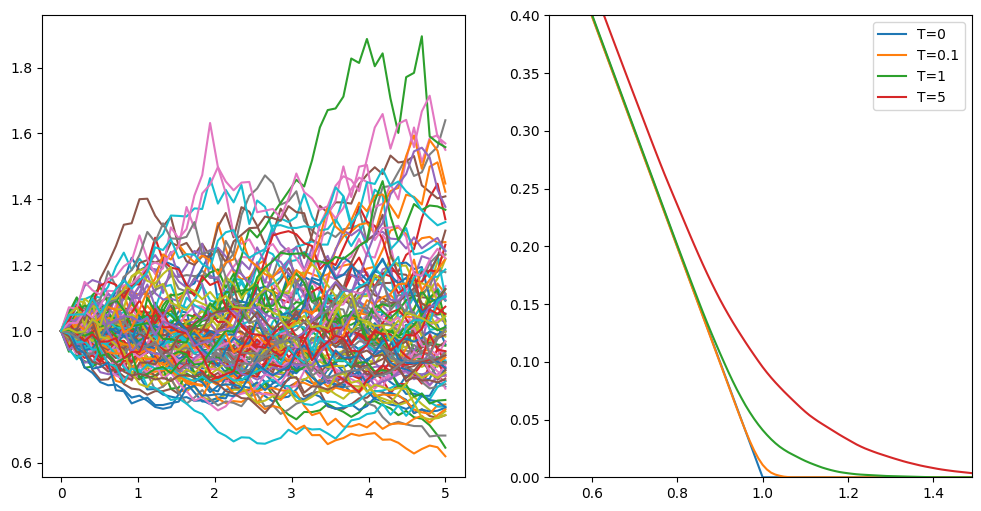
\includegraphics[width=0.8\linewidth]{addons/cev_sim}
\end{center}
\end{solution}

%%%%%%%%%%%%%%%%%%%%%%%%%%%%%%%%%%%%%%%%%%%%%%%%%%%
\question Compute the stochastic differential $dZ$ when
\begin{enumerate}[label=(\alph*),font=\itshape]
\item $Z(t) = \exp(\alpha t)$;
\item $Z(t) = \int_0^t g_s dW_s$ where $g$ is an adapted stochastic process;
\item $Z(t) = \exp(\alpha W(t))$;
\item $Z(t) = \exp(\alpha X(t))$ where $X$ has stochastic differential $dX(t)=\mu dt + \sigma dW(t)$ with $\mu$ and $\sigma$ constants;
\item $Z(t) = X^2(t)$ where $X$ has stochastic differential $dX(t)=\alpha X(t)dt + \sigma X(t)dW(t)$.
\end{enumerate}
\fillwithlines{3cm}

\begin{solution}
\begin{enumerate}[label=(\alph*),font=\itshape]
\item $dZ_t= \alpha e^{\alpha t}dt$;
\item $dZ_t = g(t) dW_t$;
\item by \ito formula: $dZ_t = \frac{\alpha^2}{2}Z(t)dt + \alpha Z_t W_t$;
\item by \ito formula: $dZ_t = (\alpha\mu + \frac{\alpha^2\sigma^2}{2})Z(t)dt + \alpha \sigma Z_t W_t$;
\item by \ito formula: $dZ_t = (\sigma^2 + 2\alpha)Z_t dt + 2\sigma Z_t W_t$.
\end{enumerate}
\end{solution}

%%%%%%%%%%%%%%%%%%%%%%%%%%%%%%%%%%%%%%%%%%%%%%%%%%%
\question Compute the stochastic differential for $Z$ when $Z(t) = \/X(t)$ and $X$ has stochastic differential 
\begin{equation*}
dX(t) = \alpha X(t) dt + \sigma X(t) dW(t)
\end{equation*}
\fillwithlines{3cm}
\begin{solution}
$dZ(t)=(\sigma^2 - \alpha)Z(t)dt -\sigma Z(t)dW(t)$
\end{solution}

%%%%%%%%%%%%%%%%%%%%%%%%%%%%%%%%%%%%%%%%%%%%%%%%%%%
\question Compute the stochastic differential for $Z$ when
\begin{enumerate}[label=(\alph*),font=\itshape]
\item $Z(t) = \int_0^t e^{-as}\sigma dW(s)$
\item $Z(t) = e^{at}\int_0^t e^{-as}\sigma dW(s)$
\end{enumerate}
\fillwithlines{3cm}

\begin{solution}
\begin{enumerate}[label=(\alph*),font=\itshape]
\item $dZ(t) = e^{-at}\sigma dW(t)$;
\item Let $Y(t)=\int_0^t e^{-as}\sigma dW(s)$ and $F(t, y)=e^{at}y$. Then $Z(t)=F(t, Y)$ and \ito formula gives
\begin{equation*}
dZ(t) = a\left\{e^{at}\int_0^t e^{-as}\sigma dW(s)\right\}dt + \sigma dW(t)
\end{equation*}
\end{enumerate}
\end{solution}

%%%%%%%%%%%%%%%%%%%%%%%%%%%%%%%%%%%%%%%%%%%%%%%%%%%
\question Solve the n-dimensional linear equation
\begin{equation*}
\begin{aligned}
dX(t) &= AX(t) dt + \sigma dW(t)\\
X(0) &= x_0
\end{aligned}
\end{equation*}
where $B$ is a d-dimensional Brownian motion, $\sigma$ is a $n\times d$-matrix and $A$ is an $n\times n$-matrix
\fillwithlines{3cm}

\begin{solution}
Using \ito formula one can check that the solution is given by
\begin{equation*}
X(t) = e^{At}x_0 + \int_0^te^{A(t-s)}\sigma dW(s)
\end{equation*}
where we have used the matrix exponential $e^{At}$ defined by
\begin{equation*}
e^{At} = \sum_{k=0}^{\infty} \cfrac{A^k}{k!}t^k
\end{equation*}
\end{solution}

%%%%%%%%%%%%%%%%%%%%%%%%%%%%%%%%%%%%%%%%%%%%%%%%%%%
\question Let $W$ be a Brownian motion and $\mathcal{F}$ the natural filtration generated by $W$. Show, using stochastic calculus, that the following processes are martingales,
\begin{enumerate}[label=(\alph*),font=\itshape]
\item $W^2(t) - t$;
\item $\exp\{\lambda W(t) - \lambda^2\frac{t}{2}\}$, where $\lambda$ is a fixed real number.
\end{enumerate}
\fillwithlines{3cm}

\begin{solution}
\ito formula gives
\begin{enumerate}[label=(\alph*),font=\itshape]
\item $d(W^2(t) - t) = 2W(t)dW(t)$;
\item $d(\exp\{\lambda W(t) - \lambda^2\frac{t}{2}\}) = \lambda\exp\{\lambda W(t) - \lambda^2t/2\}dW(t)$.
\end{enumerate}
We know that $\int_0^tX(s)dW(s)$ is a martingale if $X$ is adapted (and square integrable) so we see that the process are martingales.
\end{solution}

%%%%%%%%%%%%%%%%%%%%%%%%%%%%%%%%%%%%%%%%%%%%%%%%%%%
\question Check whether the following processes $X(t)$ are martingales (w.r.t. the natural filtration generated by $W$),
\begin{enumerate}[label=(\alph*),font=\itshape]
\item $X(t) = W(t) + 4t$;
\item $X(t) = W^2(t)$;
\item $X(t) = t^2W(t) - 2\int_0^tsW(s)ds$;
\item $X(t) = W_1(t) + W_2(t)$ where $W_1$ and $W_2$ is a 2-dimensional Brownian motion.
\end{enumerate}
\fillwithlines{3cm}

\begin{solution}
\ito formula gives the stochastic differentials 
\begin{enumerate}[label=(\alph*),font=\itshape]
\item $dX(t) = 4dt + dW(t) $;
\item $dX(t) = dt+2W(t)dW(t)$;
\item $dX(t) = t^2dW(t)$;
\item $dX(t) = W_1(t)dW_2(t) + W_2(t)dW_1(t)$.
\end{enumerate}
Since the drift term has to be zero in order for the process to be a martingale we see that the process in (a) and (b) are not martingales, while the processes in (c) and (d) are.
\end{solution}

%%%%%%%%%%%%%%%%%%%%%%%%%%%%%%%%%%%%%%%%%%%%%%%%%%%
\question Supoose that $X$ satisfies the SDE
\begin{equation*}
dX(t) = \alpha X(t)dt + \sigma X^{\beta}(t)dW(t)
\end{equation*}
where $\alpha, \sigma, \beta$ are constants and $W$ is a Brownian motion.
\begin{enumerate}[label=(\alph*),font=\itshape]
\item Determine the constants $a, b, c$ such that $Y(t) = \exp\{-a X^b(t) + ct\}$ is a martingale;
\item compute $\mathbb{E}[X(t)]$ when $\beta =1/2$;
\item compute $\text{Var}[X(t)]$ when $\beta =1/2$.
\end{enumerate}
\fillwithlines{3cm}

\begin{solution}
\begin{enumerate}[label=(\alph*),font=\itshape]
\item $a=2\alpha/(b\sigma^2)$, $b=2(1-\beta)$ and $c=ab(b-1)\sigma^2/2$;
\item $\mathbb{E}[X(t)] = x_0e^{\alpha t}$;
\item $\text{Var}[X(t)] = \frac{x_0\sigma^2}{\alpha}(e^{2\alpha t}-e^{\alpha t})$.
\end{enumerate}
\end{solution}

%%%%%%%%%%%%%%%%%%%%%%%%%%%%%%%%%%%%%%%%%%%%%%%%%%%
\question Let $h(t)$ be a deterministic function and define the process $X$ by
\begin{equation*}
X(t) = \int_0^t h(s) dW(s)
\end{equation*}
Show that $X(t)$ is normally distributed with 
\begin{equation*}
\mathbb{E}[X(t)] = 0, \quad \text{Var}[X(t)] = \int_0^t h^2(s) ds
\end{equation*}
by showing that 
\begin{equation*}
\mathbb{E}[\exp\{i u X(t)\}] = \exp\left\{-\frac{1}{2}u^2 \int_0^t h^2(s) ds\right\}
\end{equation*}
\fillwithlines{3cm}

\begin{solution}
Fix $u$ and put $Z(t)=\exp (iuX(t))$. Using \ito formula gives
\begin{equation*}
Z(t) = Z_0 - \int_0^t \cfrac{1}{2}u^2h_s^2Z_s ds + \int_0^t iuh_sZ_sdW_s
\end{equation*}
Taking expected value and solving the resulitng ODE for $m(t)=\mathbb{E}[Z(t)]$:
\begin{equation*}
\frac{dm}{dt} = -{1}{2}u^2h^2(t)m(t), \quad m(0)=1
\end{equation*}
yields the result.
\end{solution}

%%%%%%%%%%%%%%%%%%%%%%%%%%%%%%%%%%%%%%%%%%%%%%%%%%%
\question Let $X$ and $Y$ staisfy the following system of SDE's
\begin{equation*}
\begin{cases}
dX(t) = \alpha X(t) dt + Y(t)dW(t), \quad X(0) = x_0\\
dY(t) = \alpha Y(t) dt - X(t)dW(t), \quad Y(0) = x_0\\
\end{cases}
\end{equation*}
where $x_0$ and $y_0$ are deterministic constants.
\begin{enumerate}[label=(\alph*),font=\itshape]
\item Show that $R$, defined by $R(t) = X^2(t)+Y^2(t)$ is deterministic;
\item compute $\mathbb{E}[X(t)]$ and $\text{Cov}(X(t), Y(t))$, and determine for which value of $\alpha$ the process $R$ becomes a deterministic constant.
\end{enumerate}
\fillwithlines{3cm}

\begin{solution}
\begin{enumerate}[label=(\alph*),font=\itshape]
\item \ito formula gives
\begin{equation*}
dR(t)=(2\alpha + 1)R(t)dt,\quad R(0)=x_o^2 + y_0^2
\end{equation*}
Hence $R(t) = (x_0^2 + y_0^2)e^{(2\alpha + 1)t}$.
\item First compute $\mathbb{E}[X(t)] = x_0e^{\alpha t}$ and  $\mathbb{E}[Y(t)] = y_0e^{\alpha t}$. The let $Z=XY$ and use \ito formula. Taking expected value gives
\begin{equation*} 
\mathbb{E}[Z(t)] = x_0y_0 + \int_0^t(2\alpha - 1)\mathbb{E}[Z(s)]ds
\end{equation*}
Solving the ODE for $m(t) = \mathbb{E}[Z(t)]$ gives 
\begin{equation*} 
m(t) = x_0y_0e^{(2\alpha - 1)t}
\end{equation*}
Using $\text{Cov}(X(t)Y(t))=\mathbb{E}[X(t)Y(t)]-\mathbb{E}[X(t)]\mathbb{E}[Y(t)]$ gives the answer
\begin{equation*} 
\text{Cov}(X(t), Y(t)) = x_oy_0e^{2\alpha t}(e^t - 1)
\end{equation*}
\end{enumerate}

\end{solution}

%%%%%%%%%%%%%%%%%%%%%%%%%%%%%%%%%%%%%%%%%%%%%%%%%%%
\question Let $X$ and $Y$ be given by
\begin{equation*}
\begin{cases}
dX(t) = \alpha X(t) dt + \beta X(t)dW_2(t), \quad X(0) = x_0\\
dY(t) = \gamma Y(t) dt + \sigma X(t)dW_1(t), \quad Y(0) = x_0\\
\end{cases}
\end{equation*}
where $\alpha, \beta, \gamma$ are constant and $W_1$ and $W_2$ are independent Brownian motions.
Compute $\mathbb{E}[X(t)Y(t)]$.
\fillwithlines{3cm}
\begin{solution}
With $Z=XY$ we have by \ito formula that
\begin{equation*}
dZ(t) = (\gamma+\alpha\sigma)Z(t)dt + (\alpha + \sigma)Z(t)dW_1(t) + \beta Z(t)dW_2(t)
\end{equation*}
Integrating and taking expectation gives
\begin{equation*}
\mathbb{E}[Z(t)] = Z_0 + (\gamma+\alpha\sigma)\int_0^t\mathbb{E}[Z(s)]ds
\end{equation*}
Put $m(t)=\mathbb{E}[Z(t)]$ we get the ODE for $m$:
\begin{equation*}
\cfrac{dm}{m} = (\gamma+\alpha\sigma)m(t),\quad m(0)=x_0y_0
\end{equation*}
Solving this ODE we get $\mathbb{E}[Z(t)]=x_0y_0e^{(\gamma+\alpha\sigma)t}$
\end{solution}

%%%%%%%%%%%%%%%%%%%%%%%%%%%%%%%%%%%%%%%%%%%%%%%%%%%%%%%%%%%%%%%%%%%%%%%%%%%%%


\end{questions}
\end{document}
